\documentclass[12pt]{article}
\usepackage{amsmath}
\usepackage{geometry}
\usepackage{setspace}
\usepackage{graphicx}
\usepackage{fancyhdr}
\geometry{a4paper, margin=1in}
\setlength{\parindent}{0pt}
\setstretch{1.5}
\usepackage{booktabs}

\begin{document}

% -------------------------------------------------------------
% COVER PAGE
% -------------------------------------------------------------
\begin{titlepage}                                             % Create cover page
\pagestyle{empty}                                             % No headers or footers on cover
\centering                                                    % Centre all contents on cover page

% University logo or other image

\includegraphics[width=0.4\textwidth]{UoD_Engineering.jpg} \\
\vspace{20mm}                                                 % Vertical space

% Title and subtitle
{\LARGE \textbf{AIBM4 Autonomous Material Mover}} \\[10pt]  % Main title
 

\vspace{5mm}\hrule\vspace{15mm}                               % Horizontal rule below title

% Insert image with caption for the material mover
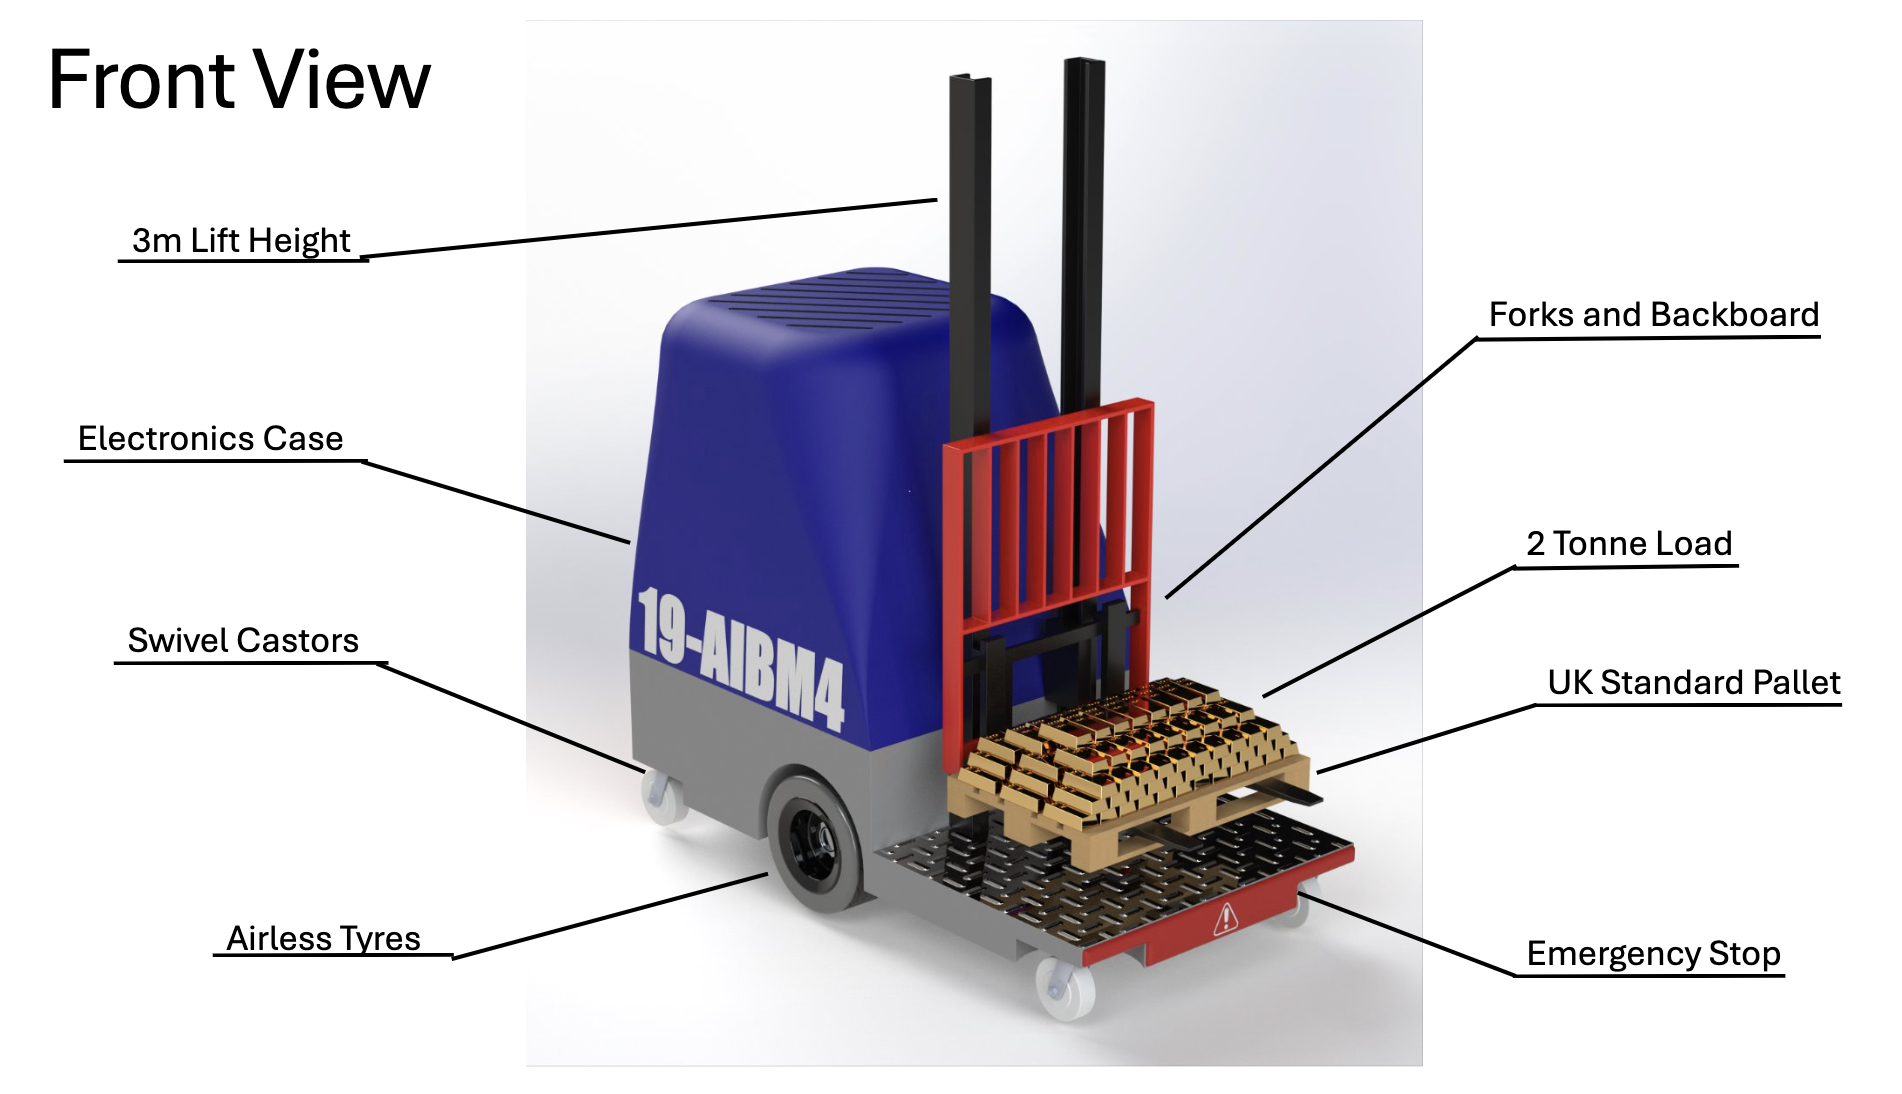
\includegraphics[width=1\textwidth]{Screenshot 2024-11-14 at 17.52.59.png}  \\  % Image of material mover
\vspace{5mm}
\textit{Figure: Front View of the 19-AIBM4 Autonomous Material Mover} \\

\vspace{20mm}                                                 % Additional space before authors

% Title and author block
{\large Anna Wigmore, Abi Wright, Louis Nangle, Will Woodward, Jiaxi Wang, Henry Billing} \\ \vspace{2mm} % The author names
{Supervisor: Aissa Ikhlef, Bill Maxwell } \\[10pt]  % The supervisor
{\small The University of Durham \\ \today}                   % University and date at bottom

\end{titlepage}
 





% -------------------------------------------------------------
% FRONTMATTER
% -------------------------------------------------------------
\tableofcontents                                              % Add table of contents
\newpage
% -------------------------------------------------------------
% MAIN CONTENT
% -------------------------------------------------------------
 

% Additional content and structure here as needed

  
 

\section{Problem Statement}

Have efficient, automated material handling within industrial environments is important, specifically factories. As industries strive toward the fourth industrial revolution, automation across all aspects of manufacturing and logistics becomes crucial. However, one area that remains largely dependent on manual labor is the transport of heavy materials and goods between supplier delivery, storage, and production or assembly areas. Conventional forklifts, whether powered by internal combustion or electricity, require human operators, which limits productivity, increases operational costs.

This design project seeks to address these challenges by developing an automated material mover capable of transporting up to two tonnes of load within a factory setting. The design must account for various elements of the factory environment, from layout to communication protocols, creating an integrated, commercially viable ecosystem for goods handling. By automating this link in the production chain, the project aims to enhance efficiency, reduce labor reliance, and offer a flexible solution adaptable to a range of factory layouts and workflows. This approach not only aligns with the push for increased automation but also positions the material mover as a disruptive solution in a market dominated by traditional, manned forklifts.





% Include the image
\begin{figure}[h!]
    \centering
    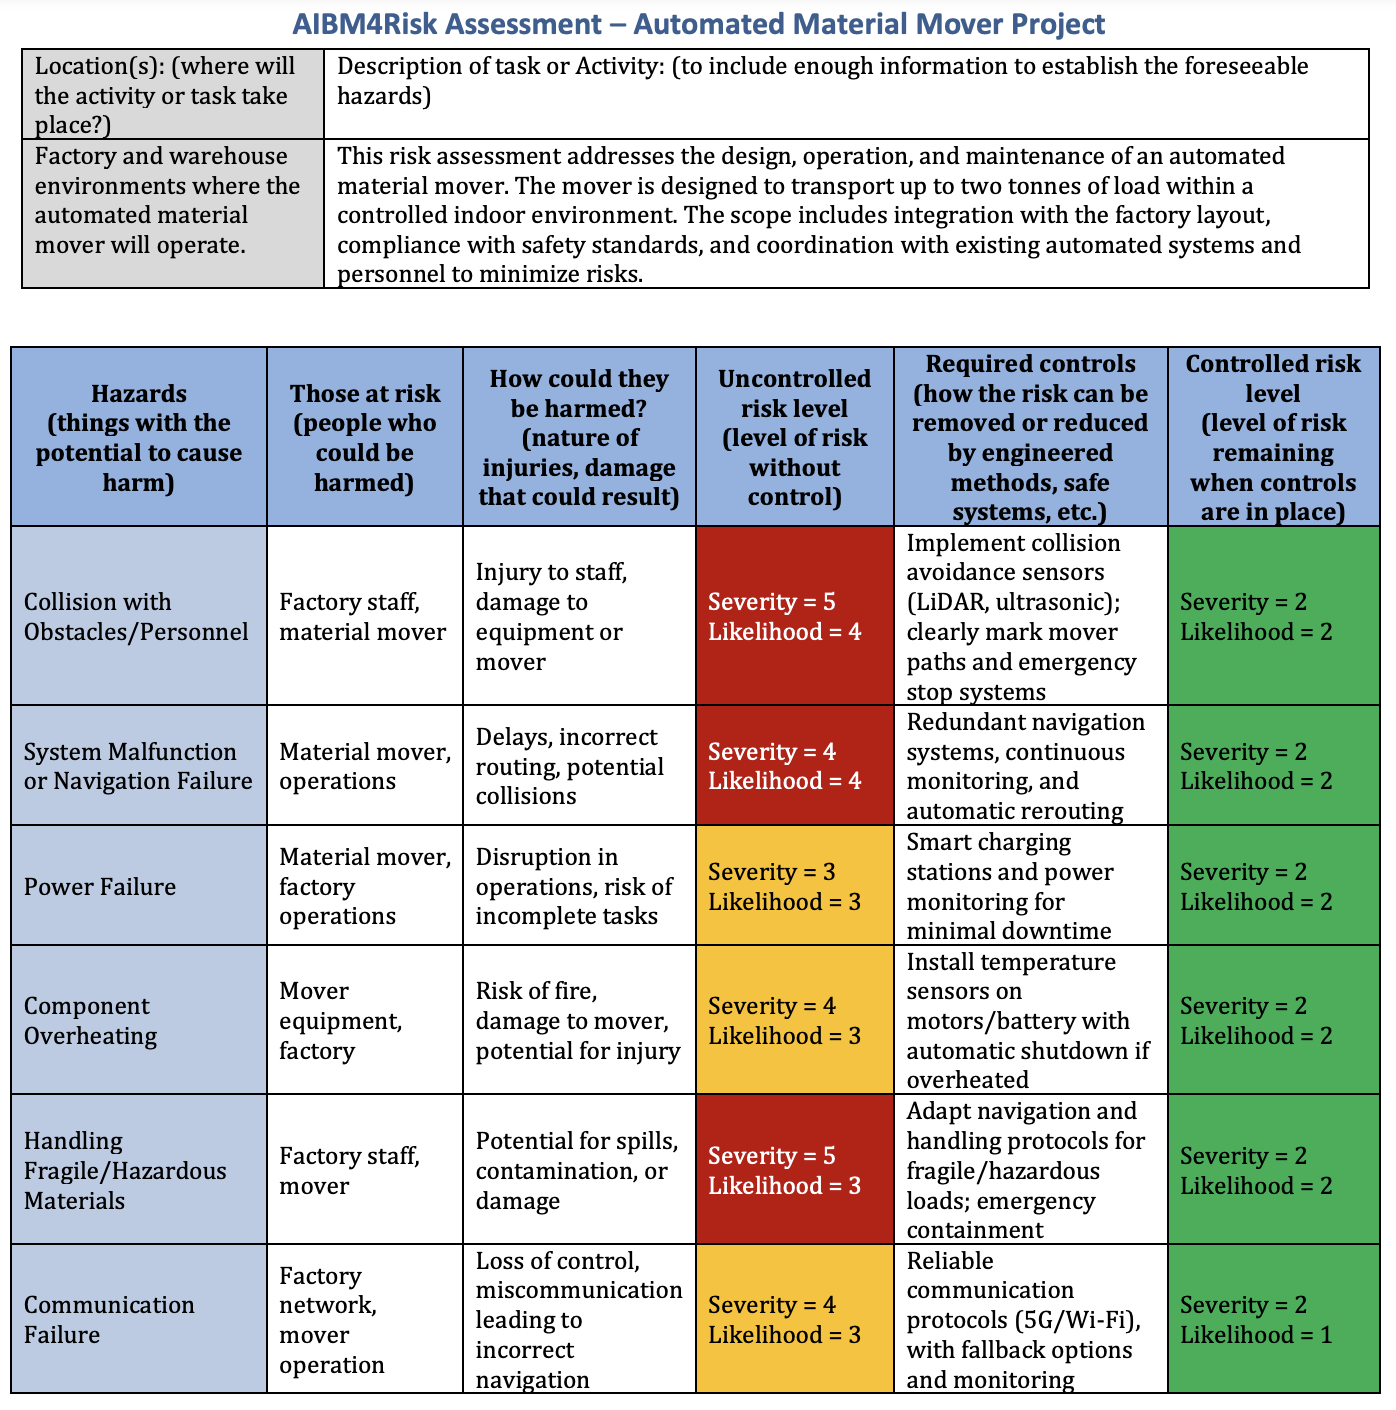
\includegraphics[width=\textwidth]{Risk_Assessment_Automated_Material_Mover_Project1.png}
     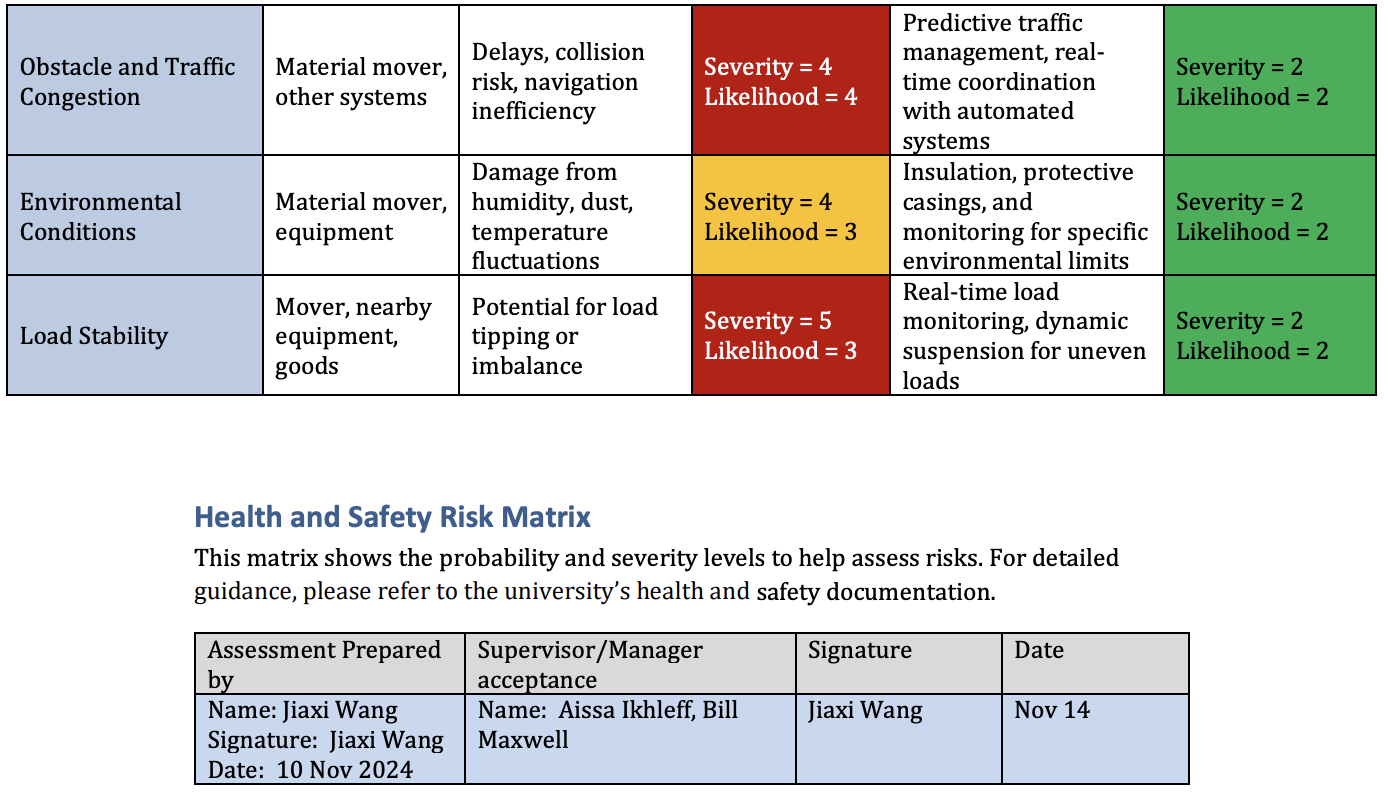
\includegraphics[width=\textwidth]{Risk_Assessment_Automated_Material_Mover_Project2.png}
    \caption{Risk Assessment – Automated Material Mover Project}
    \label{fig:risk_assessment}
\end{figure}

 

% Include the image
 \section{Introduction and Project Scope}
 the estimated budget for this project, titled AIBM4, would be £60,000. This covers labor costs at approximately £18,000 and includes material mover parts estimated at around £15,099.12, with additional allowances for wiring, software, and programming.


\begin{figure}[h!]
    \centering
    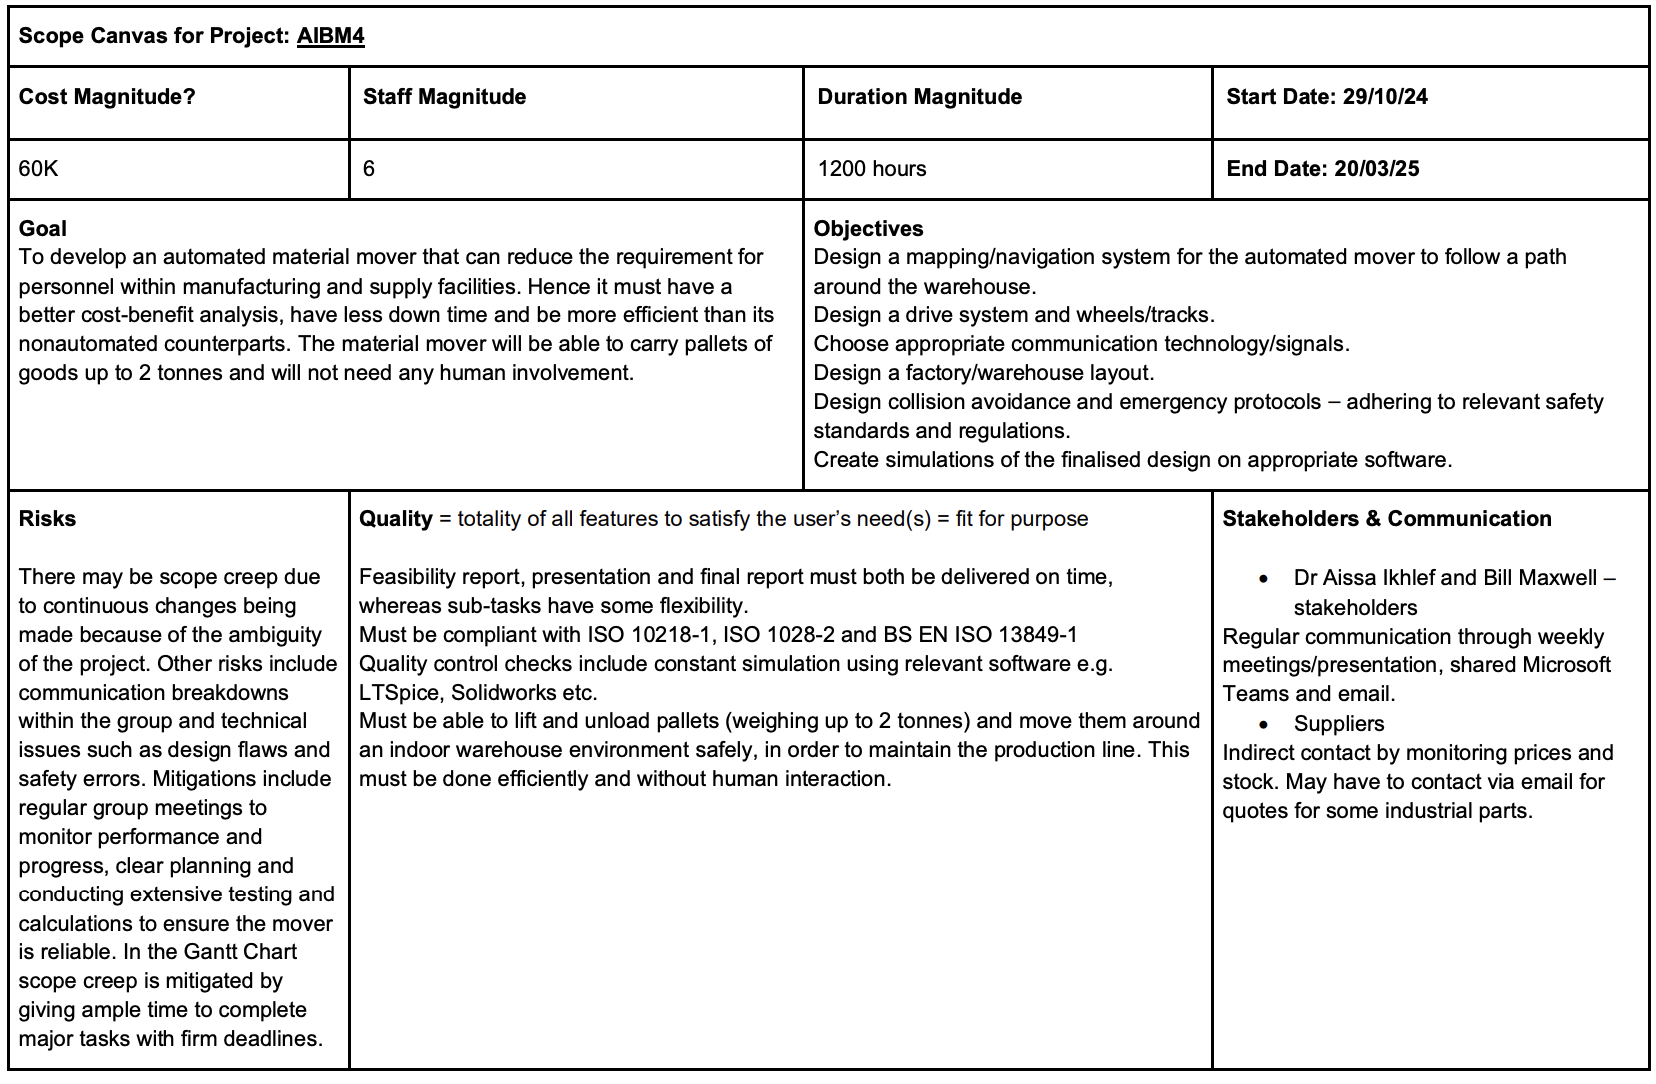
\includegraphics[width=1\textwidth]{scope1.png}
  \label{fig:Project Scope Document for AIBM4}
\end{figure}

\begin{figure}[h!]
    \centering
     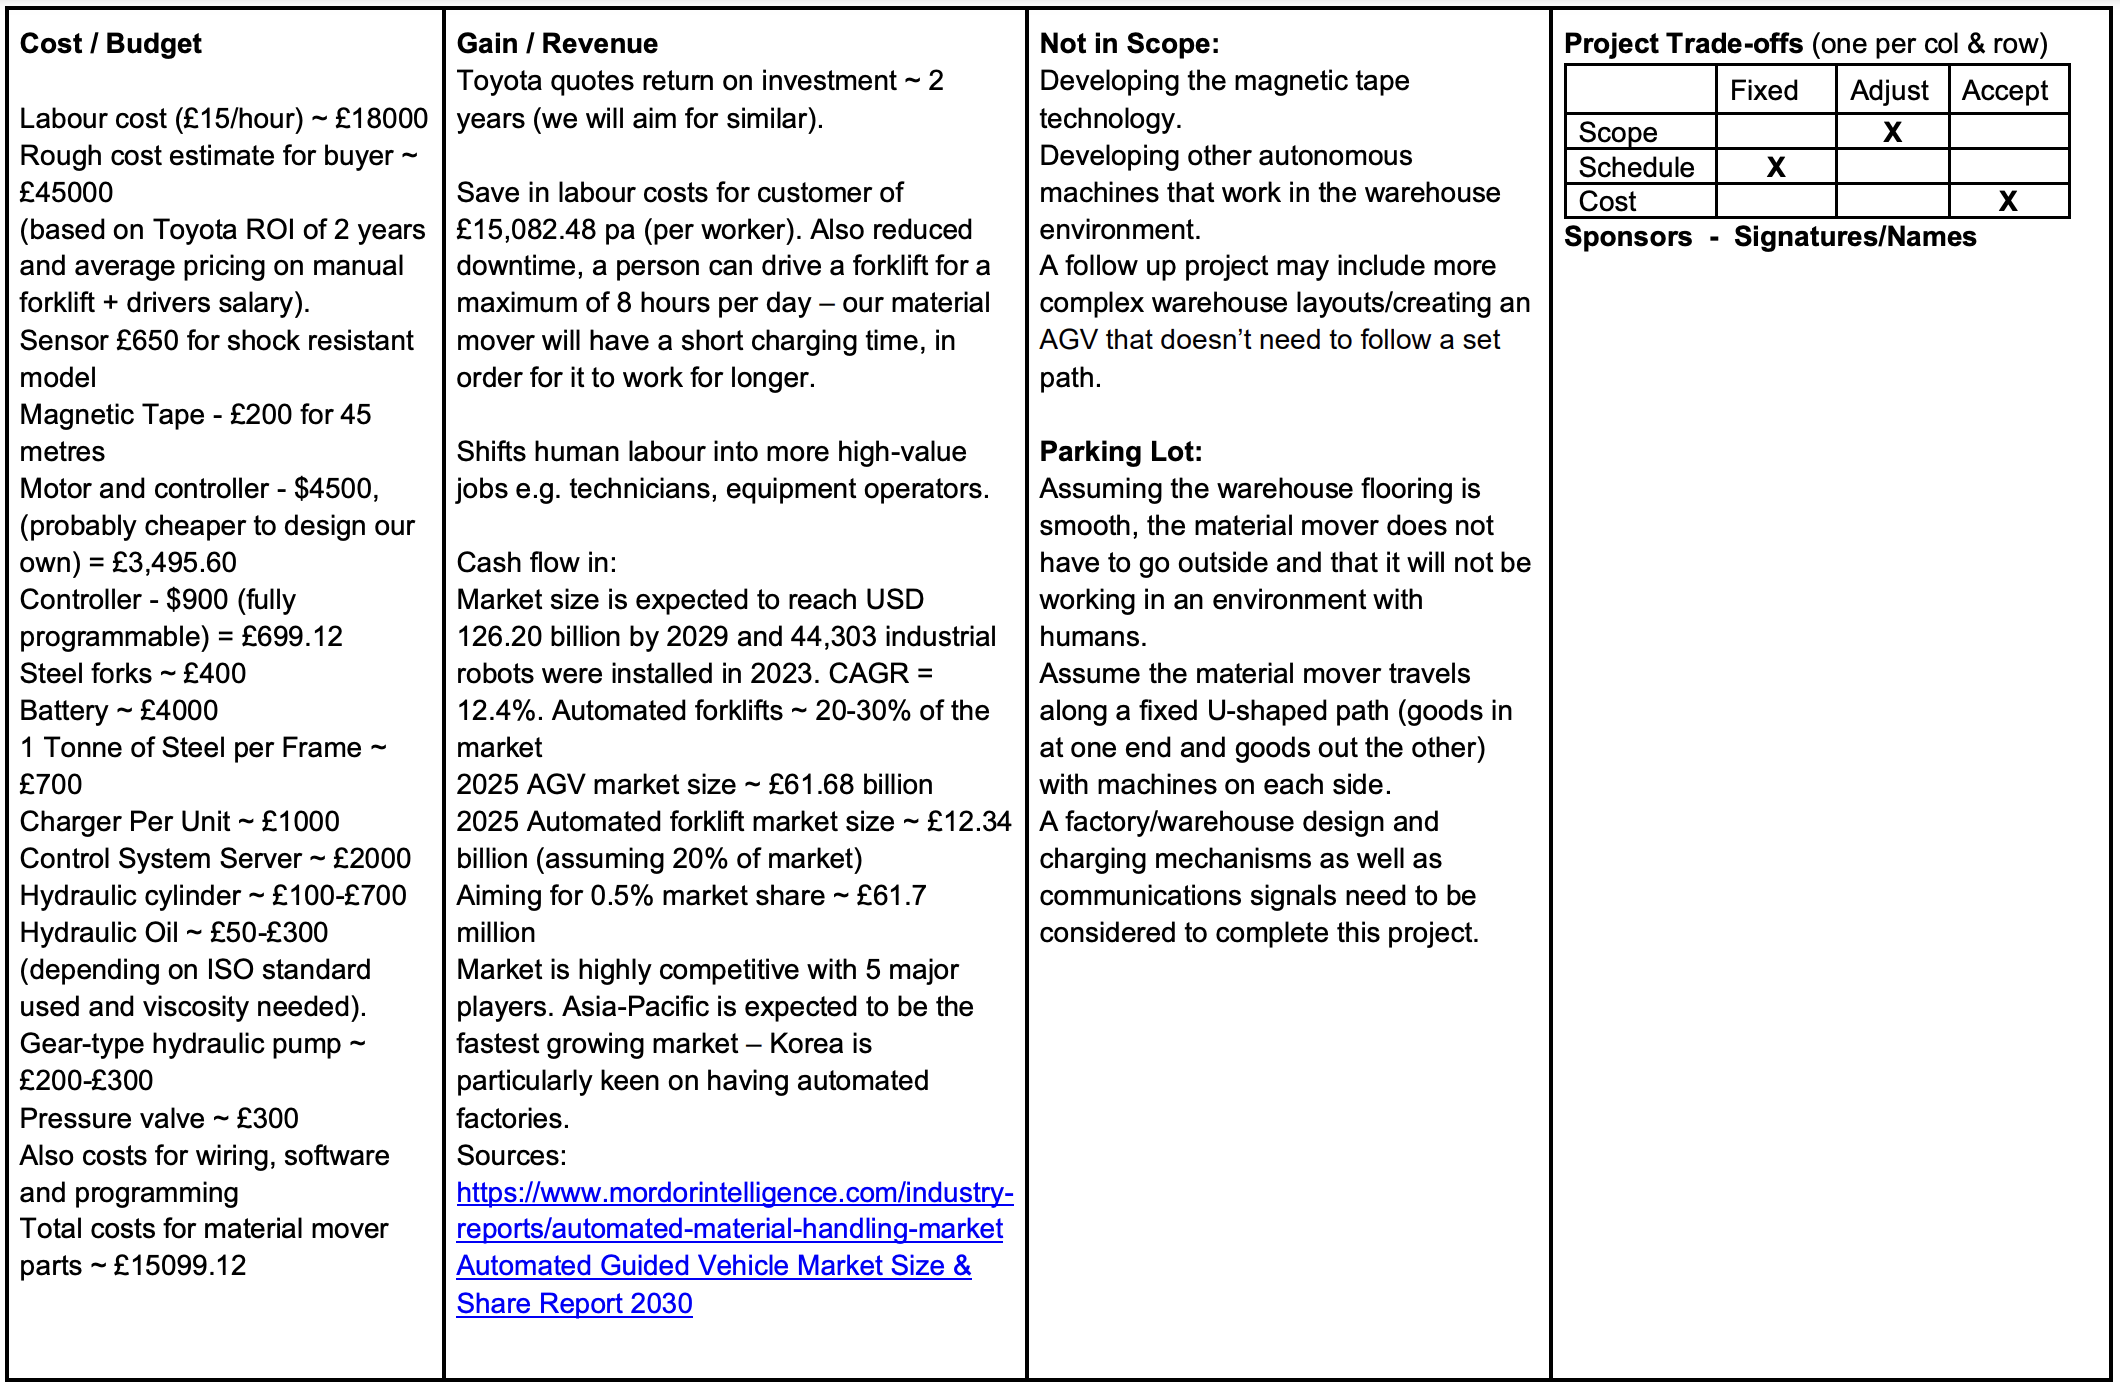
\includegraphics[width=1\textwidth]{scope2.png}
        \caption{Detailed Scope, Objectives, and Resources for Project AIBM4, focused on developing an automated material mover to enhance efficiency in manufacturing and supply facilities.}
         \label{fig:Project Scope Document for AIBM4}
\end{figure}


  \section{User Requirement Specification}


 

 
 
    \section{Concepts}
     

\begin{figure}[h!]
    \centering
     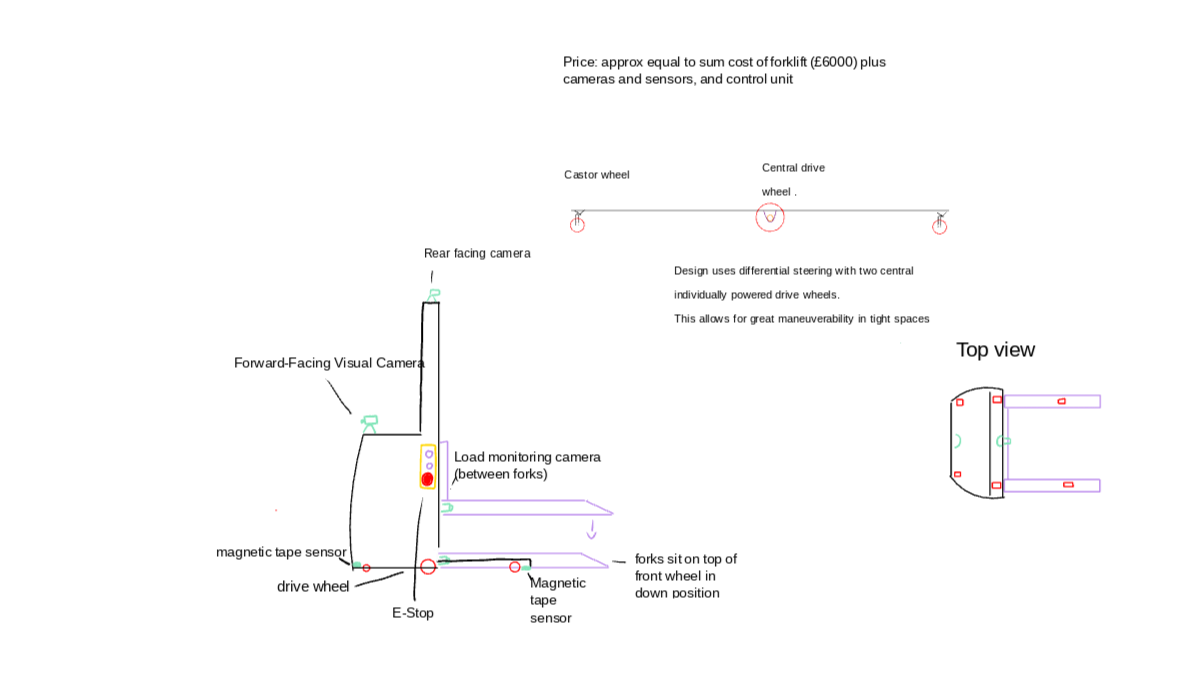
\includegraphics[width=1\textwidth]{Louis's design.png}
        \caption{Louis's design}
         \label{fig:Louis's design}
\end{figure}

\begin{figure}[h!]
    \centering
     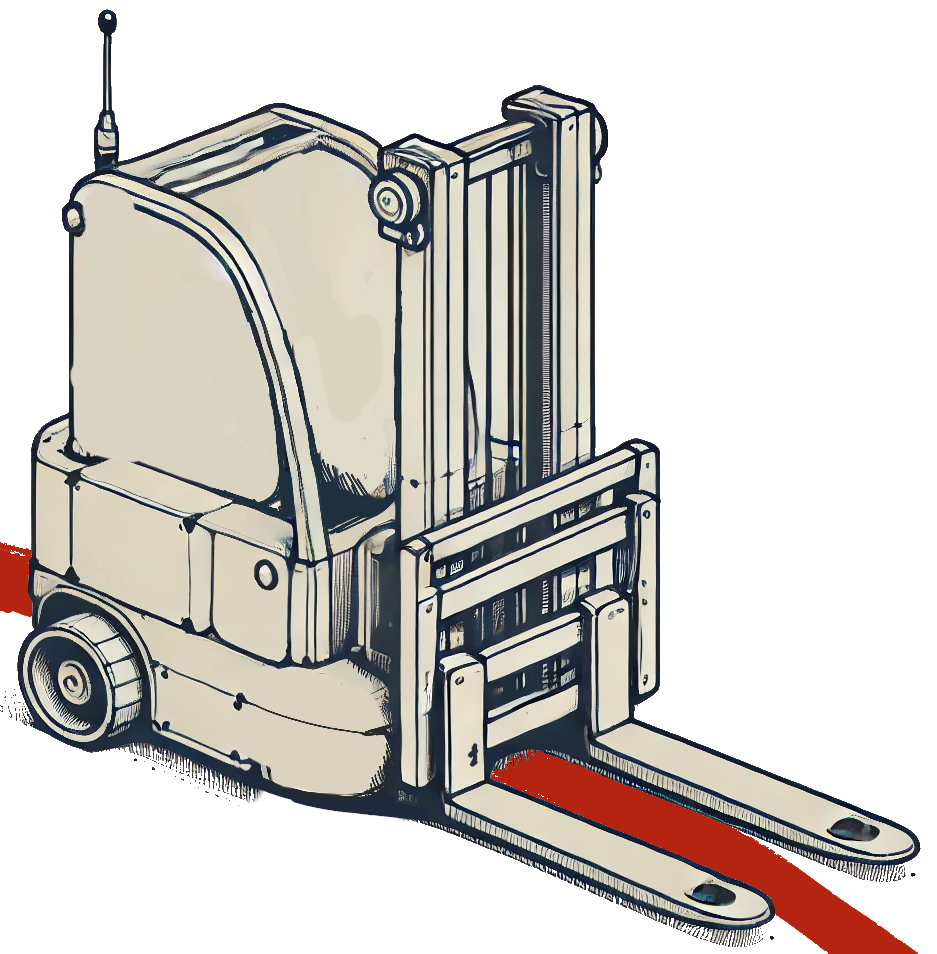
\includegraphics[width=1\textwidth]{Simple_sketch_of_an_automated_forklift_robot_with_two_wheels_at_the_back_and_one_wheel_in_the_front.png}
        \caption{Jiaxi and Abi's design}
         \label{fig:three wheel line flowing}
\end{figure}





\begin{figure}[h!]
    \centering
     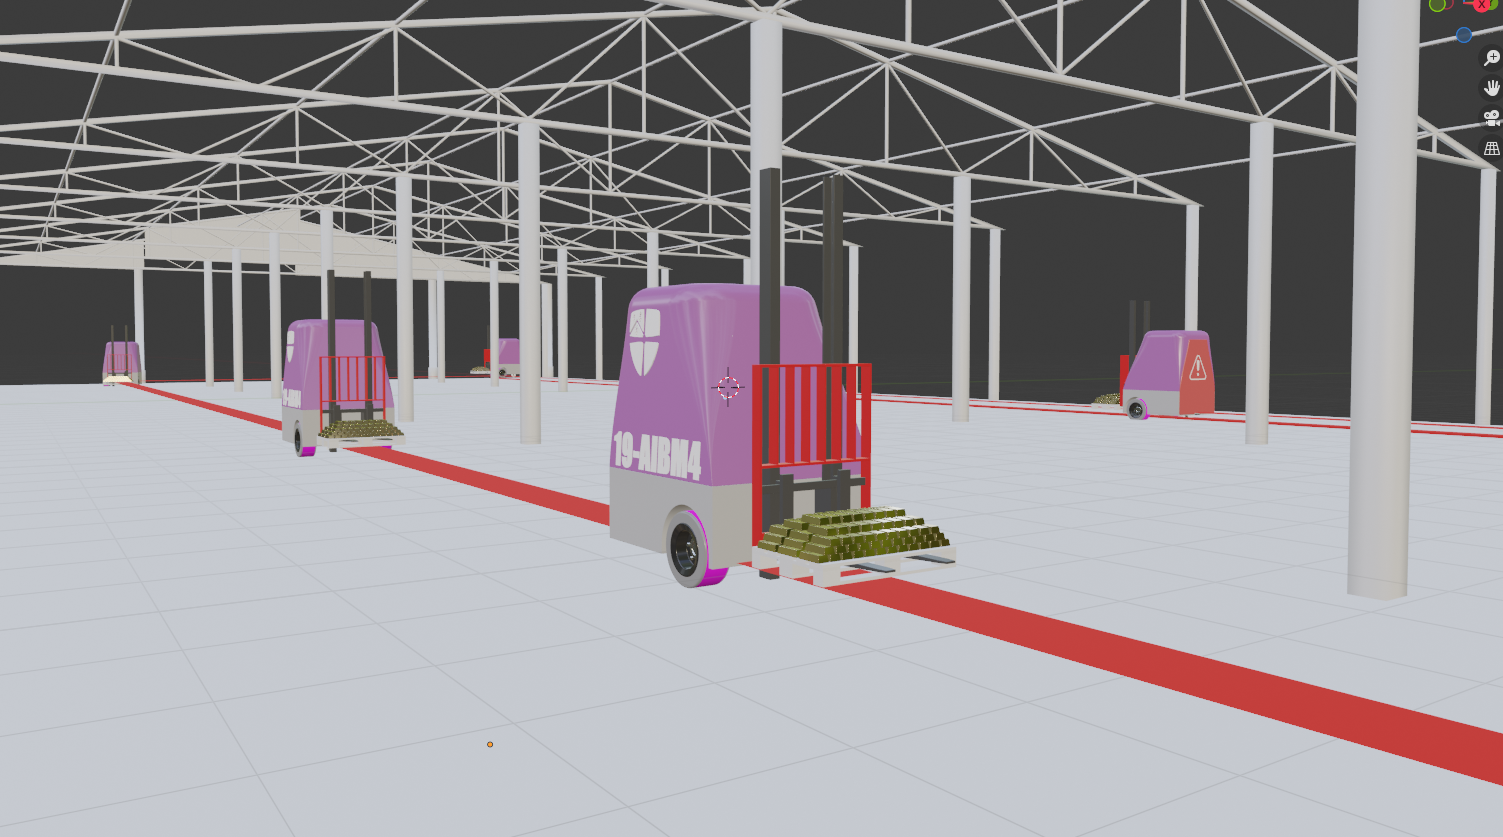
\includegraphics[width=1\textwidth]{factory layout1}
        \caption{factory layout}
         \label{fig:factory layout}
\end{figure}

\section{Three possible concepts}

\section{strengths and weaknesses of each concept}
\begin{figure}[h!]
    \centering
     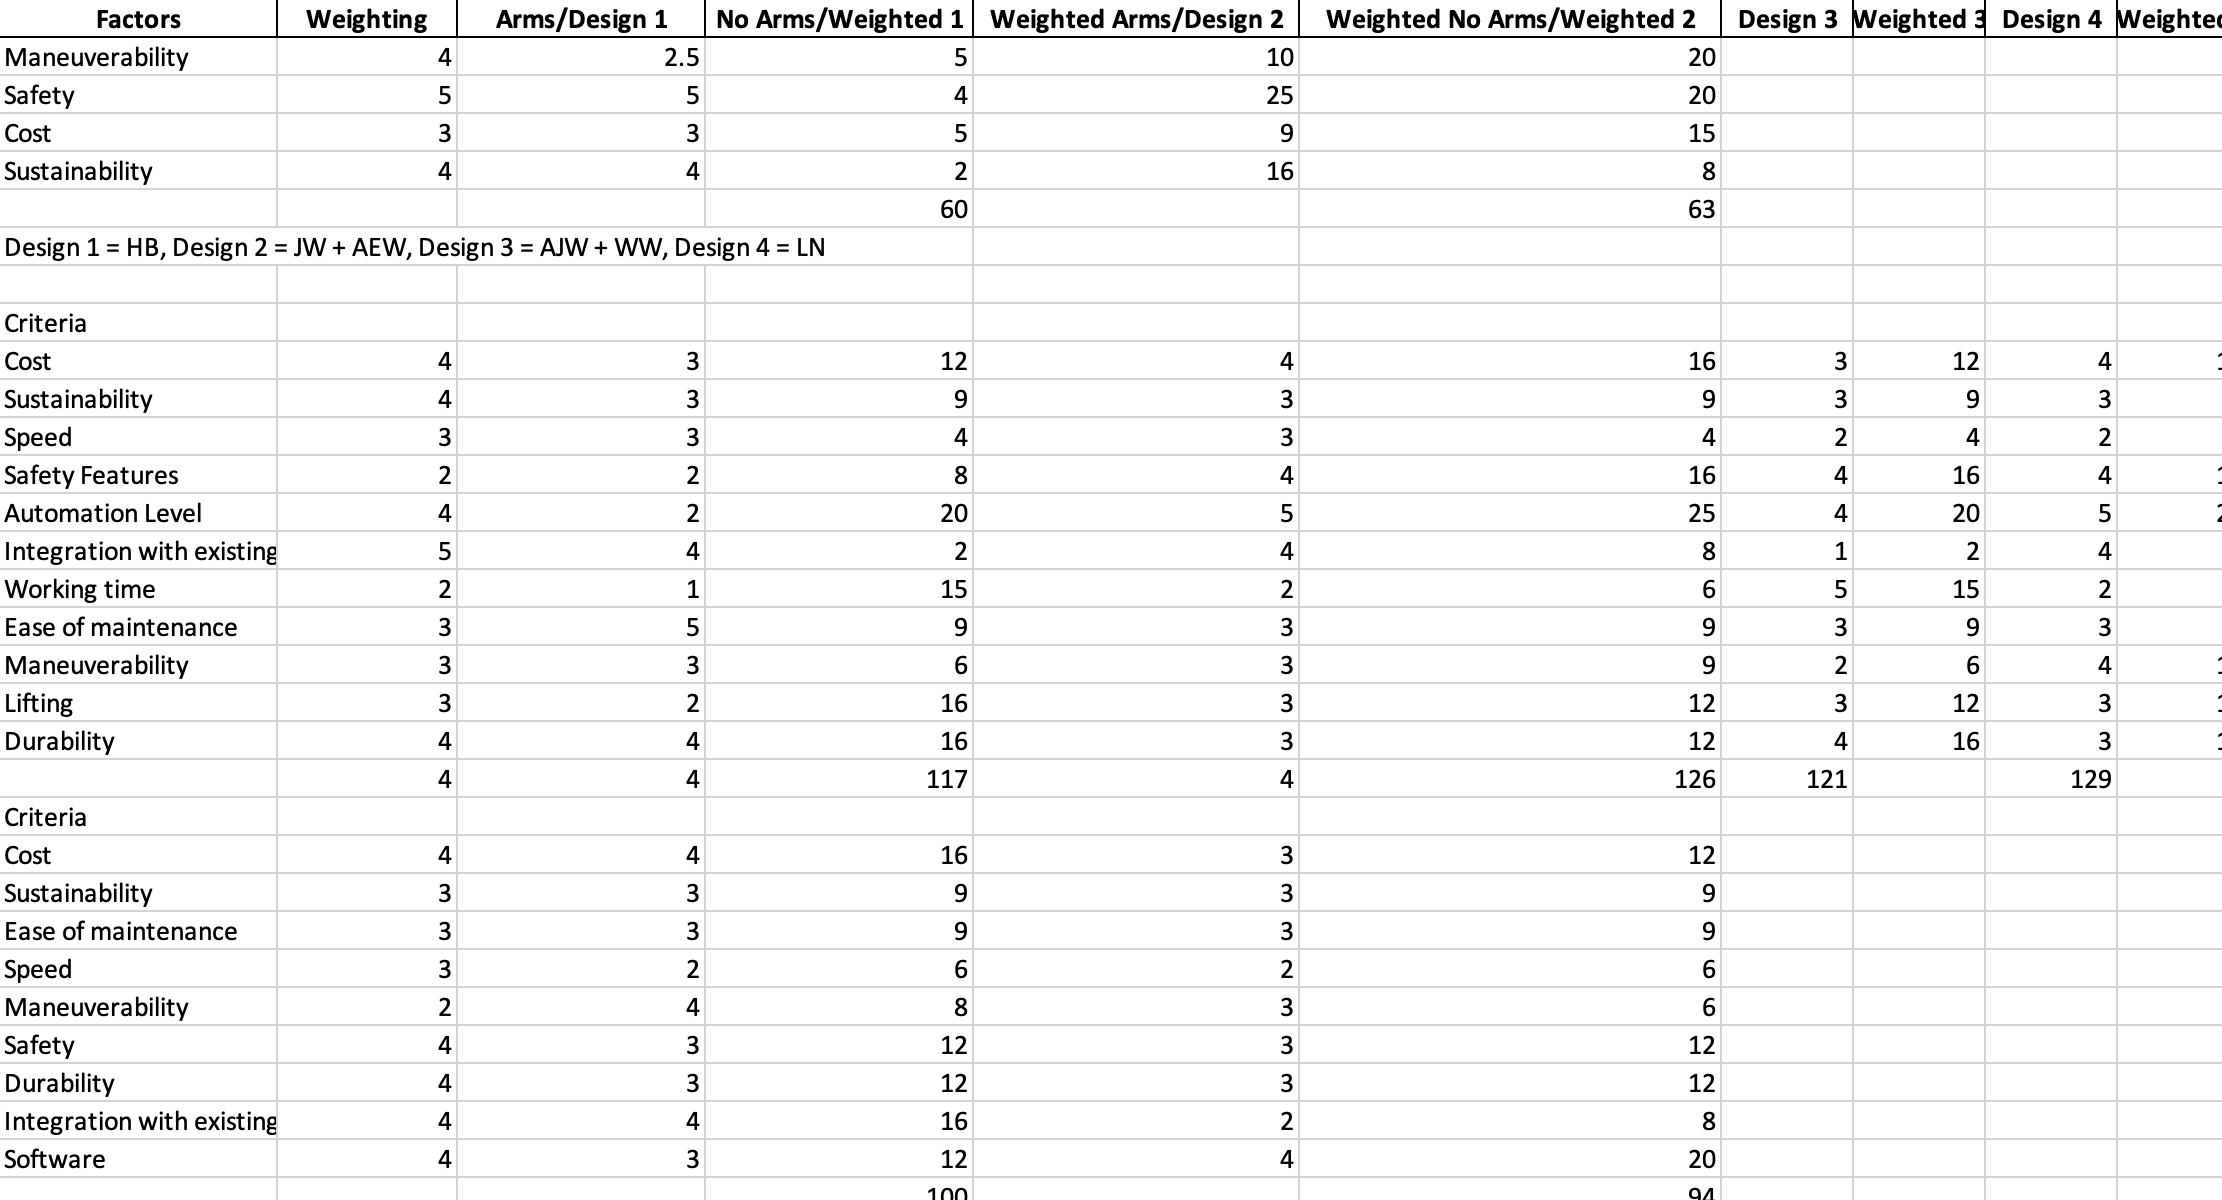
\includegraphics[width=1\textwidth]{matrix.png}
        \caption{matrix}
         \label{fig:matrix}
\begin{figure}
    \centering
    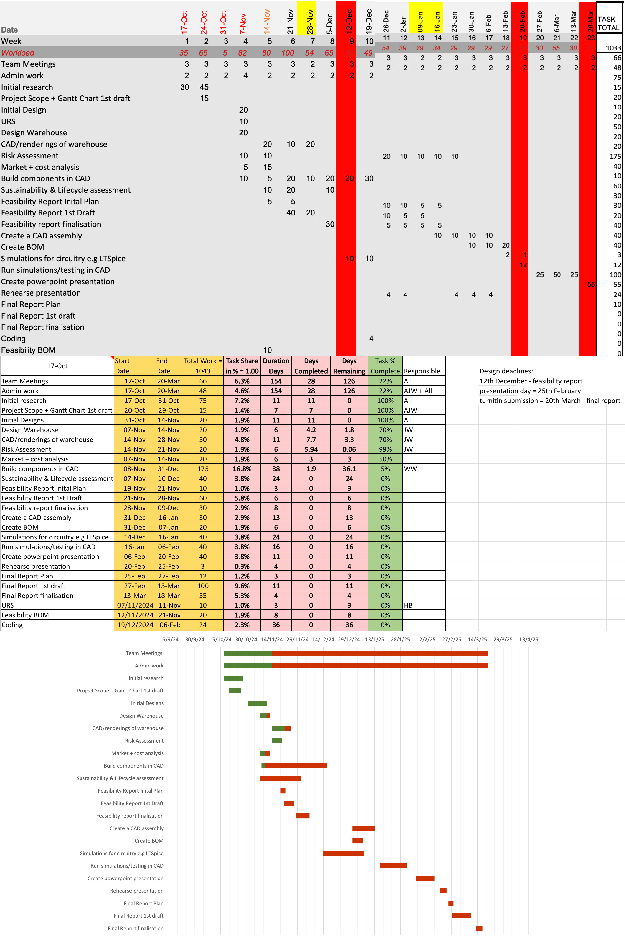
\includegraphics[width=0.5\linewidth]{gantt chart.png}
    \caption{Enter Caption}
    \label{fig:enter-label}
\end{figure}
\end{figure}
 
 
\section{Chosen Solution(s)}


\begin{figure}[h!]
    \centering
     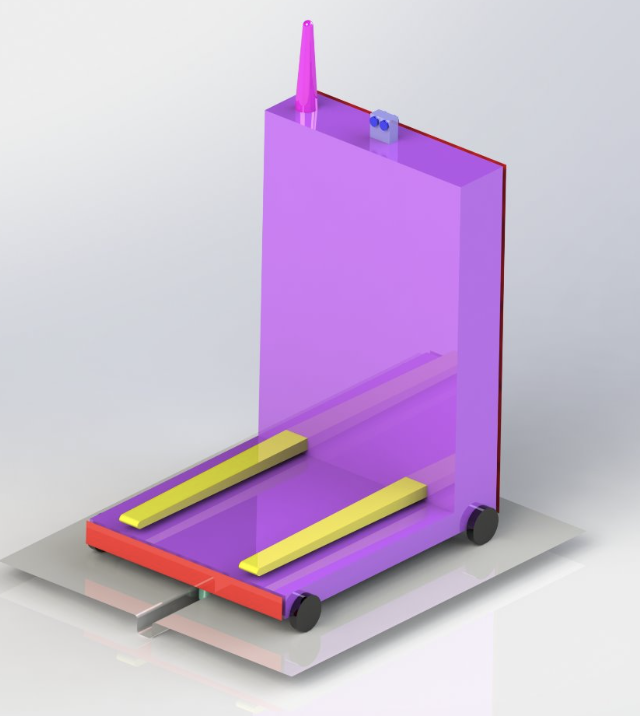
\includegraphics[width=1\textwidth]{anna&will's design.png}
        \caption{design idea}
         \label{fig:design ide}
\end{figure}


\section{Project Schedule}
Summarise what your group intends to do and when you intend to do it.
\begin{figure}[h!]
    \centering
     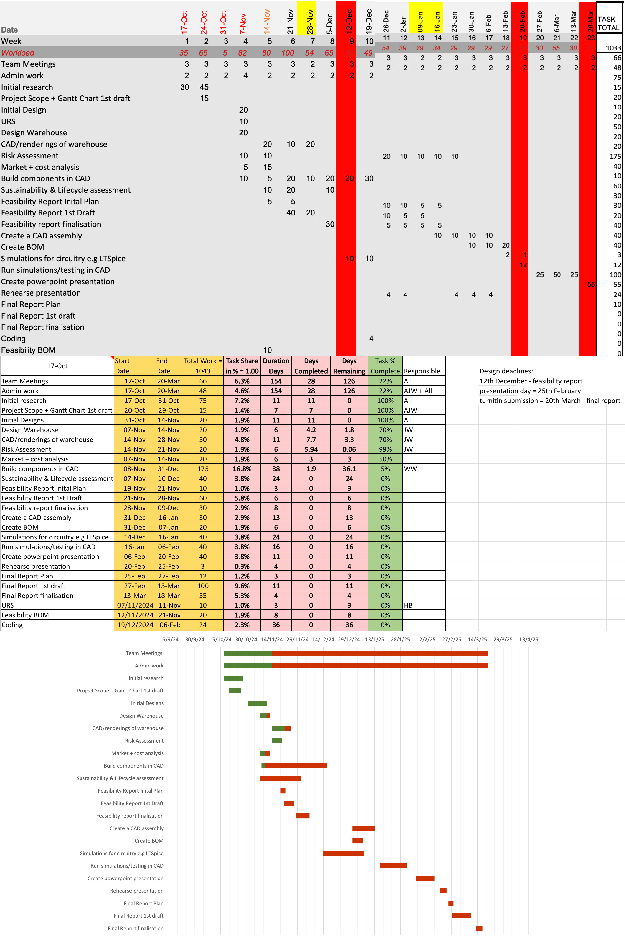
\includegraphics[width=1\textwidth]{gantt chart.pdf}
        \caption{gantt chart}
         \label{fig:timeline}
\end{figure}

Define which solution(s) should be taken forward and investigated, and why.

    \begin{itemize}
        \item Include the expected cost of the product and your basis for suggesting that cost.
        \item For larger projects, present a commercial business case, including finance and marketing information for the chosen solution.
    \end{itemize}

\section*{Expected Product Cost and Basis for Suggestion}

The total estimated cost of producing the automated material mover is approximately \textbf{£60,000}. This estimate includes labor, components, and overhead costs related to design, assembly, and testing.

\subsection*{1. Labor Costs}
\begin{itemize}
    \item \textbf{£18,000} (based on £15/hour over 1200 hours)
\end{itemize}

\subsection*{2. Material Costs}
Core components for the material mover include:
\begin{itemize}
    \item Sensors, Motors, Controllers, Batteries, Frame Steel, Chargers, Hydraulic Systems, and Control and Programming Elements totaling approximately \textbf{£15,099.12}.
\end{itemize}

\subsection*{3. Manufacturing Overhead}
\begin{itemize}
    \item Estimated overheads related to assembly, testing, and quality assurance add \textbf{£10,000} to ensure compliance with regulatory and quality standards.
\end{itemize}

\subsection*{4. R\&D and Simulation Software}
\begin{itemize}
    \item Estimated cost of \textbf{£2,000} to cover software licenses, simulations, and testing tools (e.g., LTSpice, Solidworks).
\end{itemize}

\subsection*{5. Contingency}
\begin{itemize}
    \item A contingency of \textbf{£4,900.88} is set aside for unforeseen expenses or additional materials required for modifications or safety enhancements.
\end{itemize}

The overall estimated cost is calculated by summing these elements, resulting in a \textbf{total expected cost of £60,000}.

\section*{Commercial Business Case for Automated Material Mover (Project AIBM4)}

\subsection*{Financial Analysis}

\textbf{Revenue Potential}:
\begin{itemize}
    \item \textbf{Market Size and Penetration:} The automated forklift market is projected to reach \textbf{£12.34 billion by 2025}. Achieving a modest \textbf{0.5\% market share} results in a projected revenue of \textbf{£61.7 million}.
    \item \textbf{Projected ROI:} Aiming for a similar \textbf{2-year ROI} as Toyota’s automated solutions, this mover could attract customers interested in fast payback periods.
\end{itemize}

\textbf{Customer Savings}:
\begin{itemize}
    \item \textbf{Labor Savings:} Automating pallet movement saves companies approximately \textbf{£15,082.48 per year per worker}, reducing dependency on human-operated forklifts.
    \item \textbf{Reduced Downtime:} The mover requires shorter charging periods, allowing it to operate longer shifts than human operators, thus maximizing productivity.
\end{itemize}

\subsection*{Competitive Advantage}
\begin{itemize}
    \item Unlike traditional forklifts, the automated material mover provides a \textbf{consistent, uninterrupted workflow} that maximizes uptime.
    \item \textbf{Safety Compliance:} Adherence to ISO 10218-1, ISO 1028-2, and BS EN ISO 13849-1 standards ensures market readiness and compliance, appealing to industries with strict safety regulations.
\end{itemize}

\subsection*{Marketing Strategy}

\textbf{Target Markets}:
\begin{itemize}
    \item Manufacturing Facilities, Supply Chain \& Logistics Companies
    \item \textbf{Geographic Focus:} Expansion in \textbf{Asia-Pacific}, particularly South Korea.
\end{itemize}

\textbf{Positioning}:
\begin{itemize}
    \item The mover is positioned as an \textbf{affordable yet advanced automated solution} for facilities aiming to reduce labor dependency while improving operational efficiency.
\end{itemize}

\textbf{Marketing Mix}:
\begin{itemize}
    \item \textbf{Product:} A 2-ton capacity automated mover with collision avoidance and safety features.
    \item \textbf{Price:} Competitive pricing, targeted at \textbf{£45,000 per unit} for a 2-year ROI model.
    \item \textbf{Promotion:} Focus on digital platforms and trade shows targeting manufacturing and logistics industries, emphasizing ROI and cost savings.
    \item \textbf{Place:} Direct sales to facilities and distributors in high-growth regions, with a focus on \textbf{Asia-Pacific}.
\end{itemize}

\subsection*{Risk Management and Mitigation}

\textbf{Scope Creep}: Clear task allocations, regular progress assessments, and firm deadlines will help mitigate scope creep.

\textbf{Quality and Safety Standards Compliance}: Continuous simulation and quality checks throughout development ensure compliance with necessary ISO standards.

\textbf{Communication Barriers}: Consistent updates via Microsoft Teams and email will address potential communication breakdowns.


\begin{figure}[h!]
    \centering
     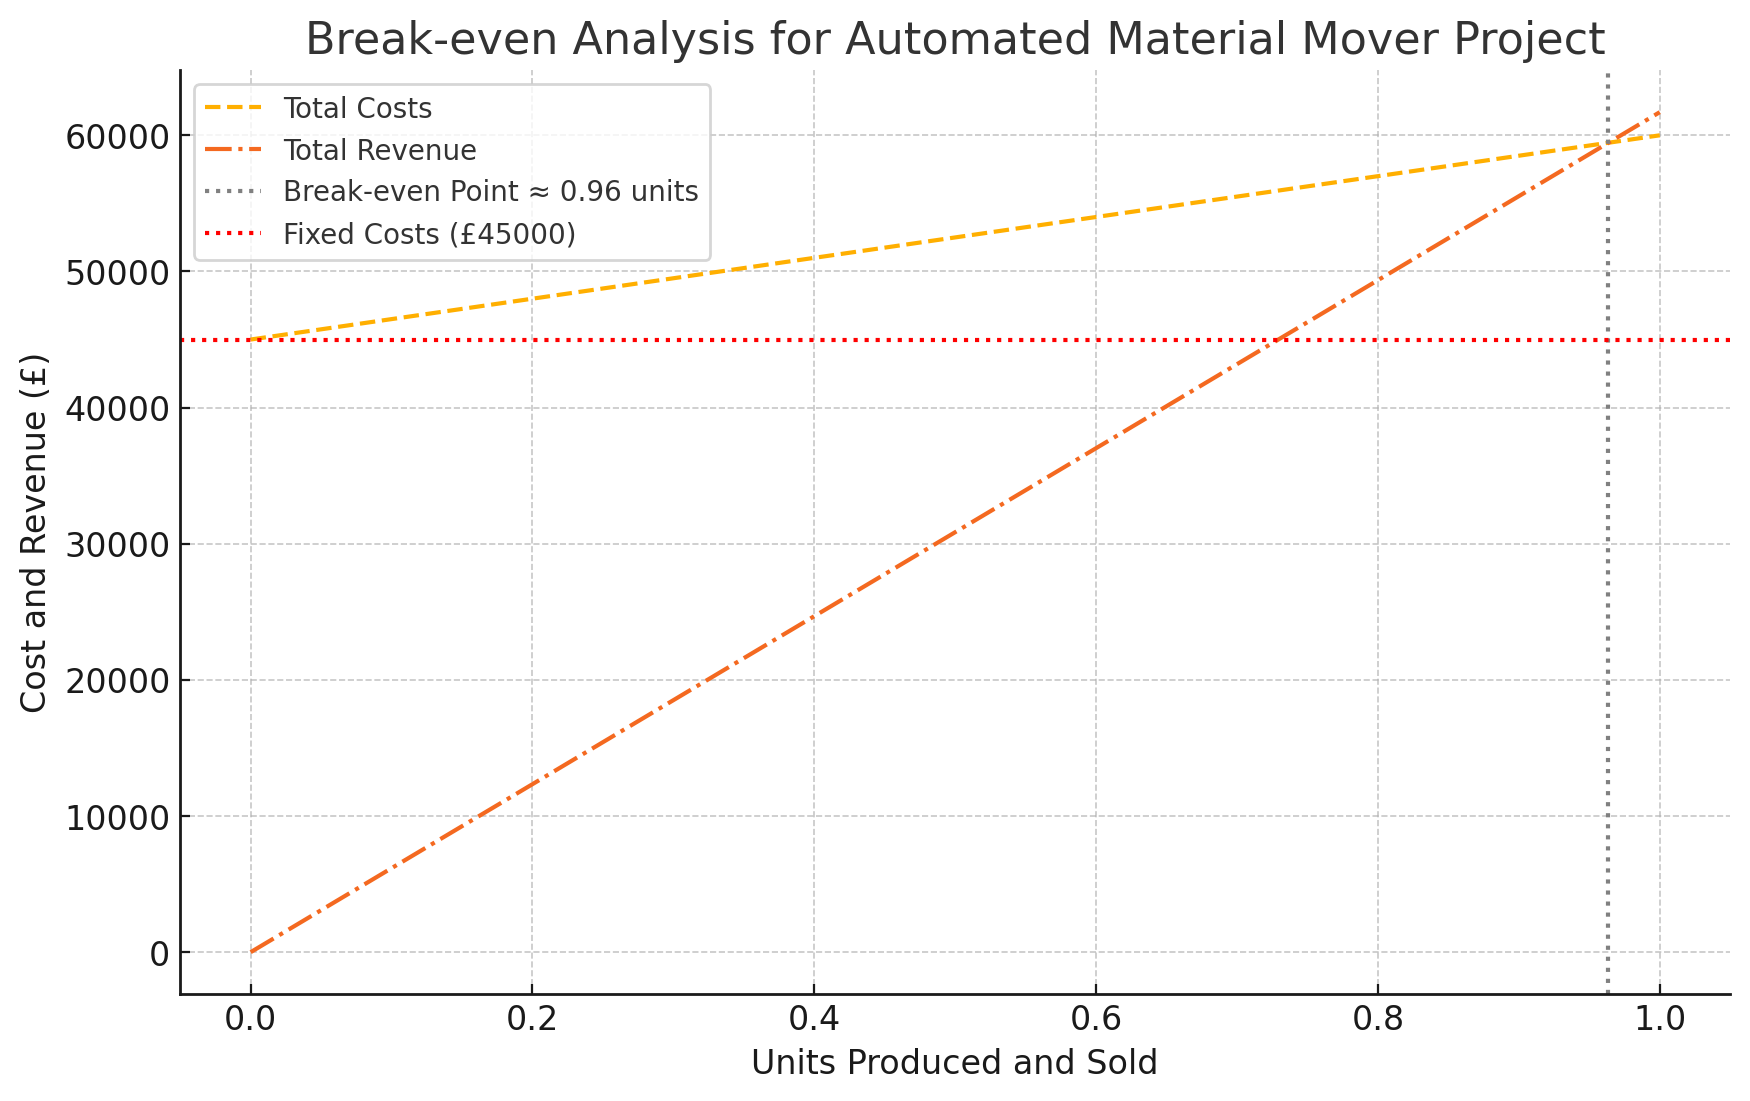
\includegraphics[width=1\textwidth]{breakeven.png}
        \caption{breakeven.png}
         \label{fig:timeline}
\end{figure}



\section{Recommendations / Conclusions}
    \begin{itemize}
        \item In light of your initial studies, should the URS be modified?
        \item Should the project proceed?
        \item Summarise your proposal/analysis in a concise format (e.g., one sentence).
    \end{itemize}
 
 
\section{References}



\section{Appendices}
 
 
\end{document}
